\chapter{Architecture, Design, and Methods}
\label{method}

The code base of SKMF is written entirely in Python
\cite{python},
with Python 3.4 used as the active interpreter throughout development. This allows the code to be portable and forward-facing enough that it should be easily maintainable. The underlying architectural pattern used is model-view-controller (MVC). This pattern lends itself well to Web applications that utilize a backend datastore. Development followed the security development lifecycle (SDL) for Agile, as prescribed by Microsoft
\cite{secdevlifecycle}.
The Agile approach that was attempted is test-driven development (TDD), although project development veered heavily from this desired approach. For the most part, development stayed along the guidelines set out in the original project plan. Implementation details and justification for several design decisions are provided in the following sections.


\section{Developing With Modern Python}
\label{method:python}

Python was chosen as the development language for SKMF because the sole developer has some familiarity with Python development, the Python project has excellent documentation, and the Python interpreter makes Python applications highly portable. Python 3.4 was chosen as the target version because the widely deployed version 2.7 is no longer supported by upstream development and version 3.5, although currently considered stable, had not reached wide adoption at the time the SKMF project was started. As of this writing, version 3.4 is the stable version of Python on both Gentoo Linux, the primary environment of the developer, and Debian Linux, which has wide adoption amongst Linux users. Adhering to Python 3.4 compatibility ensures that the project can be easily maintained.

There are also some data structures that are particularly easy to work with in Python. Sets are useful when a collection should not contain any duplicates. They are especially useful when comparisons must be made between the contents of multiple collections, such as the intersection or the difference. Dictionaries, referred to in some other object-oriented programming languages as maps, are also quite versatile. The key needs to be a hashable datatype, but the value can be any Python object. This is convenient, for example, to hold a structure of RDF triples where the subject URI is the key and the rest of any triples pertaining to that subject are stored in another data structure as the value. Such a pattern is used extensively within SKMF, modeled after the Turtle serialization format for RDF and the JSON structure of SPARQL responses. Figure
\ref{skmf-triple}
shows this structure as a tree format.

\begin{figure}[h]
\singlespace
\begin{verbatim}
{<subject_uri>|<subject_label>:
    {`type': `uri'|`pfx'|`label',
     `value':
        {<predicate_uri>|<predicate_label>:
            {`type': `uri'|`pfx'|`label',
             `value':
                [{`type': `uri'|`pfx'|`label'|`literal',
                  `value': <object_uri>|<object_label>|<xml_literal>,
                  `xml:lang': <lang_string>,
                  `datatype': <xml_datatype>
                }]
            }
        }
    }
}
\end{verbatim}
\caption[Structure of a triple in SKMF]
 {\narrower The outer dictionary is keyed off of RDF subjects, identified by URI or label for query results. The corresponding value is a dictionary with only two entries: `type' to indicate the form of the subject and `value' to point to the rest of the triples, stored in another dictionary. This dictionary is similar in structure to the outer dictionary, only keyed off of RDF predicates. The inner dictionary for predicate values is similar to the one for subject values, except that the `value' key corresponds to a list of RDF objects stored as simple dictionaries. The object dictionary most closely matches the SPARQL query result specification, while the outer dictionaries extrapolate that form to resemble the more terse Turtle serialization style.
 }
\label{skmf-triple}
\end{figure}



\section{Semantic Model-View-Controller}
\label{method:mvc}

MVC is a popular architectural pattern when working with relational databases. Typically, a schema is developed in the database and some objects are designed around the schema to form the model. The view can be implemented with any interface that suits the necessary task, often some form of dynamic Web page rendering. This leaves the controller to perform all of the program logic and pass data between the model and the view. When a graph-based datastore with a dynamic schema is used instead, the problem requires a different approach
\cite{semanticwebprogram}.
Since the only two well-known object RDF model (ORM) modules for Python, RDFAlchemy
\cite{rdfalchemy}
and SuRF
\cite{surf},
are written for Python 2.7 and do not support Python 3, the object model for SKMF was implemented from scratch.


\subsection{Modeling Around RDF}
\label{method:orm}

When data are represented as a directed graph, as with RDF, it is possible for the model of the data to change as data are added and removed. This makes it difficult to maintain a schema and nearly impossible to enforce one. Two approaches are employed by SKMF to address this issue. First, a basic schema is hard-coded into the application to support some common RDF types and some features specific to the application. Second, the application utilizes parsers that allow users to define and extend virtually any custom schema.

A prime example of a hard-coded schema in SKMF is the `User' class. A user is treated like any other RDF resource, except that it is expected to have some known properties set and it may have other optional properties that get special treatment. One property that a user must have in the current version of SKMF is `skmf:hashpass', which is a salted hash of the user's password used for authentication. Note that in this notation `skmf:' is shorthand for the SKMF namespace, or the full URI where `hashpass' is defined. The only optional property of users that receives special treatment is `foaf:name', which is displayed in some parts of the Web interface. This is also an example of incorporating an external schema by using the `foaf' namespace
\cite{foaf}
instead of defining a custom property in the local namespace.

Custom schema generation is supported by the model code of SKMF. This is possible because of the generic manner in which resources are represented and the ability to limit SPARQL statements to specified named graphs. It would be possible, for instance, to define a schema using a collection of triples that describe how resources in that schema should behave, then place that collection in a named graph that is loaded by the controller component to be parsed for rendering appropriate forms for user interaction. The prototype user interface of SKMF does not, however, reveal this functionality to the user. Although, the Web interface does make use of a hidden schema to manage users and restrict user creation to an administrative user.

In order to better support system scaling, SKMF does not manipulate RDF directly. That task is left to a SPARQL endpoint, which is expected to be capable of handing the user's data storage needs. To speak with the SPARQL endpoint, queries are constructed from the aforementioned SKMF data structure for RDF triples, along with some extra information to help form and scope the query. SPARQL does not have the same concept of prepared statements as modern relational database systems, so queries are formed as string literals. This requires a number of parsers to generate different components of the query, depending upon the query type. For instance, a typical query statement first assembles the list of variable labels, then puts together the desired named graphs as a series of `FROM' statements, then forms the body of the query, which may require forming a set of `OPTIONAL' clauses that are used by SKMF to retrieve human readable labels whenever they are available. Finally, the processed segments are placed into a template for the appropriate query type, as depicted in Figure
\ref{sparql-template}.
Figure
\ref{sparql-statement}
illustrates a fully formed SPARQL statement.

\begin{figure}[ht]
\singlespace
\begin{verbatim}
{prefix}
SELECT DISTINCT {labels}
{graphs}
WHERE {{
  {body}
  {optional}
}}
\end{verbatim}
\caption[Template for SPARQL query statements]
 {\narrower This template outlines a general SPARQL query. `prefix' is replaced by the prefix lines from the active configuration. The other tags are replaced by generated string literals.
 }
\label{sparql-template}
\end{figure}

\begin{figure}[!ht]
\singlespace
\begin{verbatim}
PREFIX rdf: <http://www.w3.org/1999/02/22-rdf-syntax-ns#>
PREFIX rdfs: <http://www.w3.org/2000/01/rdf-schema#>
PREFIX xsd: <http://www.w3.org/2001/XMLSchema#>
PREFIX skmf: <http://example.com/skmf#>

    SELECT DISTINCT ?email ?person_label ?person ?email_label
    FROM <http://example.com/skmf>
    WHERE {
      skmf:www skmf:managedby ?person .
      ?person skmf:emailaddress ?email .
      OPTIONAL { ?email rdfs:label ?email_label . }
      OPTIONAL { ?person rdfs:label ?person_label . }
    }
\end{verbatim}
\caption[Generated SPARQL query statement]
 {\narrower SPARQL query statement formed by populating a template with values assembled by SKMF. This query asks for the person who manages the www resource and an email address. The `OPTIONAL' statements ask for human readable labels, if available.
 }
\label{sparql-statement}
\end{figure}


\subsection{Views and Control With Flask}
\label{method:flask}

Numerous Web frameworks are available for Python. The Flask framework
\cite{flask}
was selected for SKMF due to multiple factors. First, it is a full-stack Web framework that is modularized to avoid excessive overhead from unused functionality. Second, Flask more closely follows Python programming principles and better supports REST APIs than Django
\cite{django},
which is a very popular Web framework for Python. While SKFM is not specifically designed to be RESTful
\cite{restful},
it could be made to support a RESTful API at a later time. Third, Flask is available through a BSD license, making it more viable than a GPL-licensed framework for a project that may not be released under the same terms. Finally, Flask is extensively documented, even though some of the sanctioned modules are not.

The Web framework is relied upon to provide many of the security features desired of SKMF. Flask-WTF
\cite{flask-wtf}
automatically handles HTML filtering of input to mitigate cross-site scripting and it provides for use of synchronizer tokens to mitigate cross-set request forgery. Flask-Bcrypt
\cite{flask-bcrypt}
is used to generate a salted hash of user passwords that are stored in place of the plain text. Flask-Login
\cite{flask-login}
manages user sessions and authorization tokens, as well as providing a mechanism for directing unauthenticated users away from protected views. Flask does not, however, provide TLS support, so that must be implemented at deployment.


\section{Security Development Lifecycle in Agile}
\label{method:sdl}

Microsoft's SDL
\cite{secdevlifecycle}
prescribes an approach to software development that aids developers in identifying security and quality concerns throughout the development process. It is aimed primarily at larger development processes, but it includes recommendations for applying its key principles to an Agile development process. TDD was chosen as the Agile development approach for SKMF since the development team consisted of only a single member and since testability is one of the quality goals of SKMF. Unfortunately, it proved difficult to maintain TDD while working with Flask, so that approach primarily drove backend development.


\subsection{Identifying Security Issues in SKMF}
\label{method:threats}

One early step of the SDL is vulnerability analysis and threat modeling. The threat model for SKMF, shown in Figure
\ref{threat-model},
revealed that SKMF would have two main vectors of attack, under a certain set of assumptions. Due to its heavy reliance on the Python interpreter, it is assumed that the hosting system is running a patched version of Python with no untrusted or unmaintained modules. It is also assumed that unauthorized users cannot access the SKMF code directly. Under these assumptions, attacks may originate from the Web server or from the external SPARQL endpoint. Both of these systems are deemed to be outside of the control of SKMF.

\begin{figure}[p]
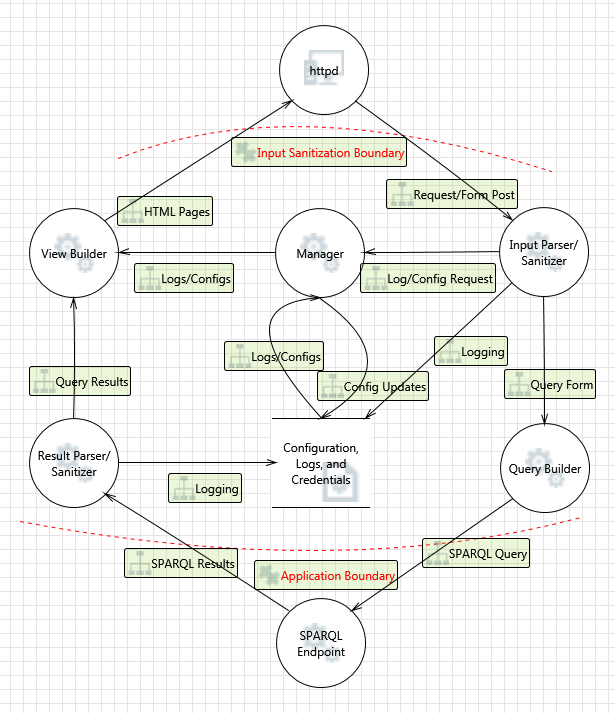
\includegraphics[width=6.5in]{threat-model}
\caption[Data flow diagram with threat boundaries]
 {\narrower Created with Microsoft Threat Modeling Tool 2016
  \cite{mstmt}.
  Data cross threat boundaries to and from the httpd Web server and the external SPARQL endpoint.
 }
\label{threat-model}
\end{figure}

Data from the Web server are considered untrusted because many of them are user supplied. The main threats identified by the model here are cross-site scripting (XSS), cross-site request forgery (CSRF), and information disclosure. An issue that was not identified by the modeling tool is injection. The first two issues are handled with Flask-WTF by always escaping text from form fields and by implementing synchronizer tokens. The third issue largely depends on secure deployment, with a secure connection between SKMF and the Web server and the use of TLS beyond that. The fourth issue requires that all input be handled safely and not passed directly to string parsers or SPARQL queries.

Steps taken within SKMF to mitigate information disclosure include handling user authentication with Flask-Login and providing the ability to scope queries and updates to specific named graphs. With a proper UI update, the use of these named graphs could allow an administrator to create a graph-based access control list for users, which could, itself, be stored in a restricted graph. Another measure to prevent information disclosure is the use of Flask-Bcrypt to provide a secure means of storing authentication tokens. Bcrypt mitigates brute-force attacks against password hashes by applying a salt to randomize the value that actually gets hashed and by using a hashing algorithm that is resource-intensive, making it very difficult to reverse. Use of a random salt also greatly reduces the likelihood that the hash of the password can be located within a rainbow table. Bcrypt does, however pose two problems for SKMF, since the hashing operations are performed on the server. The first problem is that the user's password is sent in clear text to the server. Even if it is encrypted through TLS, the clear text password is exposed for a brief time on the server and could be intercepted. The second problem is that the intensive nature of the hashing operation opens the server up to denial-of-service attacks should enough simultaneous logins be attempted. One possible solution to both problems is to offload the hashing operation onto the user's system, but that does not seem to be directly supported by Flask or any of the extensions currently used by SKMF.

Injection attacks can come in two forms. The first is format string injection, which occurs when a string formatting operation is performed directly on a user-supplied string that is assumed not to contain any string formatter tokens. The second is SPARQL injection, which occurs when a user-supplied string containing valid SPARQL escape sequences and syntax is sent to the SPARQL endpoint without being properly sanitized. Either injection attack could result in information disclosure or data corruption. To prevent format string injection, SKMF only applies the Python string format operation on static strings, like the template shown in Figure
\ref{sparql-template}.
In that template, the `body' and `optional' fields are both replaced by strings that may contain user input. That operation is performed by passing the replacement strings as arguments to the format() function, applied to the static template string. The replacement strings are constructed in a similar manner, with user input supplied as arguments to the format() function applied to some static string. Essentially, complex strings are constructed from the inside out and the format operation is only used on the outermost string at each layer, ensuring that it is never applied to a string that has been tainted by untrusted input.

SPARQL injection is more difficult to prevent. SPARQL does not offer prepared statements or parameterized queries, as do many SQL implementations, so input must be sanitized. Input sanitizing in SKMF is performed primarily by Flask-WTF, so HTML characters such as `\textless' and `\textgreater' should be escaped, making it difficult to construct a valid query injection. Since Flask-WTF handles any POST request, whether or not it was actually submitted through a Flask-WTF form, it should be difficult for an attacker to bypass the filters by crafting a special POST request. Also, SPARQLWrapper
\cite{sparqlwrapper},
which handles communication with the SPARQL endpoint, has strict requirements for how queries should be formed. SKMF forms queries as multi-line strings which means that any attempt to comment out the rest of a line during injection would most likely result in a query that SPARQLWrapper will reject. While these measures help to mitigate SPARQL injection attacks, further measures will need to be taken to properly safeguard SKMF. Ideally, a whitelisting approach will be taken when handling user input to ensure that any user-supplied field aligns with the SPARQL definition for a single variable, URI, or prefixed URI. This would ensure that only viable input could reach the SPARQL endpoint and it would provide an opportunity to alert users who have mistakenly provided invalid input.

Data from the SPARQL endpoint are considered untrusted because the security of the SPARQL endpoint is a matter of deployment. SKMF is likely to be deployed on the same host as the Web server with which it operates, but separation of duties would suggest that the datastore reside on a separate, more isolated host. This requires a secure, preferably encrypted connection between the hosts. It is, therefore, recommended that the SPARQL endpoint either support TLS or be accessible only over another secured transport, such as IPsec. The SPARQL endpoint also stores data provided by the user, which need to be retrieved. These data had to be sanitized by Flask-WTF before reaching the SPARQL endpoint, but it is still possible that something malicious is able to get through. SKMF does not, yet, sanitize outbound data.


\subsection{Attempted Test-Driven Development}
\label{method:tdd}

TDD worked well for the early model code. Simple test cases could be created and corresponding code written quite rapidly. Unfortunately, TDD did not work well for components that rely on Flask. Due to an initial lack of familiarity with the framework and, more specifically, testing within the framework, numerous difficulties were encountered when formulating test cases. Even test cases that appeared sound would frequently fail with Flask context errors. For the sake of making progress toward a functional prototype, TDD was abandoned for the duration of development.

SKMF was written with a bottom-up approach. The intention was to provide a solid foundation upon which a wide range of desired functionality could be built. It is possible, however, that a top-down approach would have worked better with TDD. In this approach, it would have been necessary to learn the proper testing procedures for Flask early on. The early test cases for validating the user facing components would then need only minor modification to verify proper support from the underlying elements that would be added later. This approach also would have ensured priority development of model code that is used by the prototype UI, allowing more time to implement demonstrable features.
